\section{Métodos de descenso de gradiente alternado}

\subsection{Factorización SVD}
Las técnicas existentes para completado de matrices están fuertemente fundamentadas en la estructura de bajo rango de las matrices que se quieren completar, lo cual genera una interdependencia entre sus entradas. Buscar explícitamente la matriz de rango bajo consistente con las entradas conocidas se puede expresar como
\begin{equation}
    \min_{Z \in \mathbb{R}^{m \times n}} \rank Z, \ \text{sujeto a} \ P_{\Omega}(Z) = P_{\Omega}(Z_0),
    \label{eqn:minrank}
\end{equation}
donde $Z_0 \in \mathbb{R}^{m \times n}$ es la matriz que se quiere reconstruir, $\Omega$ es un subconjunto de índices de las entradas conocidas y $P_{\Omega}$ es el operador que muestrea únicamente las entradas en $\Omega$.

El problema~\ref{eqn:minrank} es no convexo y generalmente NP-Completo. Uno de los enfoques más estudiados es reemplazar el rango por su versión relajada, la norma nuclear. De esta manera el problema se puede expresar como
\begin{equation}
    \min_{Z \in \mathbb{R}^{m \times n}} \norm{Z}_*, \ \text{sujeto a} \ P_{\Omega}(Z) = P_{\Omega}(Z_0),
    \label{eqn:minnuclear}
\end{equation}
donde $\norm{Z}_*$ representa la norma nuclear, dada por la suma de los valores propios de $Z$.

Muchos algoritmos para este problema involucran una descomposición SVD en cada iteración, lo cual limita su aplicabilidad para matrices muy grandes. Aquí se presenta una alternativa que evita el costo computacional de la SVD.

\subsection{Factorización de rango}
Para evitar el costo computacional de calcular la SVD, supondremos que el rango $r$ de la matriz que queremos completar es conocido y utilizaremos la descomposición mencionada en el siguiente teorema.

\begin{teorema}[Factorización de rango]
    Dada una matriz $A~\in~\mathbb{R}^{m \times n}$ de rango $r$, existen matrices $C \in~\mathbb{R}^{m \times r}$ y $F~\in~\mathbb{R}^{r \times n}$ tales que $A = CF$.
\end{teorema}

\begin{proof}
    Como $A$ es de rango $r$, existen $r$ columnas de $A$ linealmente independientes. Sea ${c_1, c_2, \ldots, c_r}$ una base del espacio generado por estas columnas y consideremos la matriz $C \in \mathbb{R}^{m \times r}$ cuyas columnas son $c_i$. Luego, cada columna de $A$ es combinación lineal de las columnas en $C$. Si $a_1, a_2, \ldots, a_n$ son las columnas de $A$, entonces existen $f_ij$ tales que
    \begin{equation*}
        a_j = f_{1j}c_1 + f_{2j}c_2 + \cdots + f_{rj}c_r,
    \end{equation*}
    para cada $j$, por lo tanto $A = CF$, donde $F = [f_{ij}]$.
\end{proof}

Basada en esta simple factorización, en lugar de resolver el problema~\eqref{eqn:minrank}, resolveremos el problema 
\begin{equation}
    \min_{X, Y} \frac{1}{2} \norm{P_{\Omega}(Z_0) - P_{\Omega}(XY)}^2_F.
    \label{eqn:minxy}
\end{equation}

Donde $\norm{\cdot}_F$ es la norma de Frobenius, definida como
\begin{align*}
    \norm{A}_F^2 &= \Angle{A, A}_F = \sum_{i,j}^{} A_{ij}^2 \\
    \Angle{A, B}_F &= \sum_{i,j} A_{ij}B_{ij} = \tr(A^T B)
\end{align*}

\subsection{Minimización alternada}
Consideremos una función $f(X, Y) \colon \mathcal{X} \times \mathcal{Y} \to \mathbb{R}$. El método de minimización alternada minimiza $f(X, Y)$ sucesivamente sobre $X$ y $Y$.

El algoritmo PowerFactorization(PF), es un algoritmo que resuelve el problema~\eqref{eqn:minxy} utilizando esta idea. 

\begin{figure}[htpb]
    \centering
    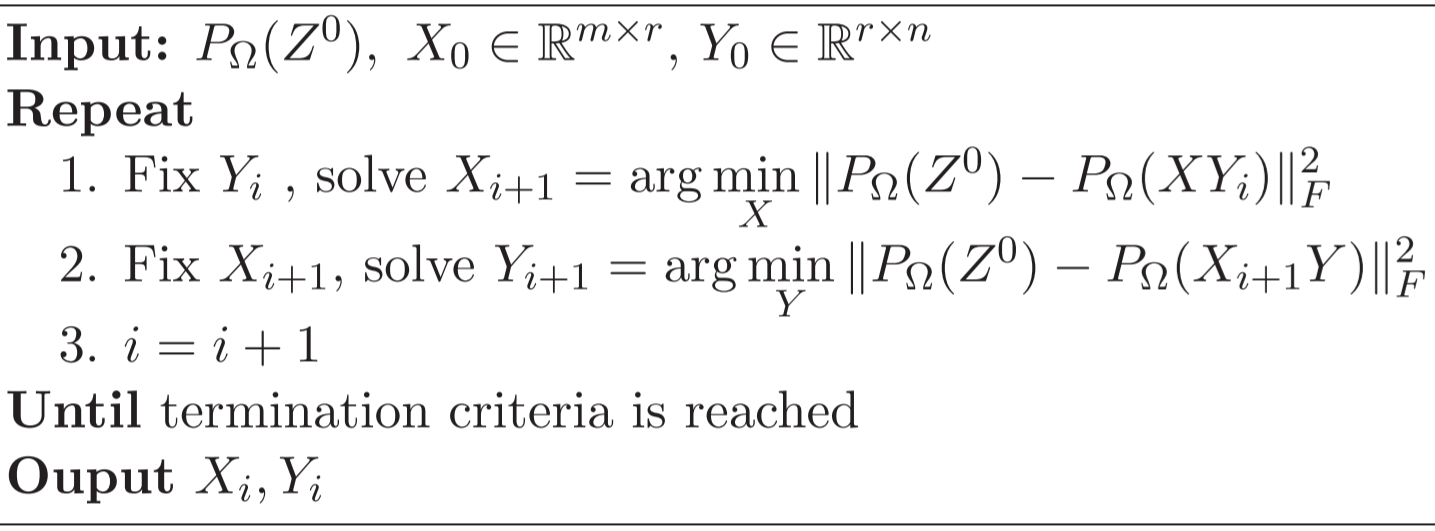
\includegraphics[width=0.95\linewidth]{../Results/ASD_Images/PF.PNG}
    \caption{PowerFactorization}\label{fig:PF}
\end{figure}

Notemos que en cada subproblema hay que resolver un problema de mínimos cuadrados, lo cual determina la complexidad del algoritmo. Existen múltiples algoritmos que se basan en este y tratan de reducir el costo computacional de mínimos cuadrados, utilizando distintas alternativas.

La alternativa que vamos a seguir para reducir el costo computacional de PowerFactorization es reemplazar resolver el problema de mínimos cuadrados por un único paso en la dirección de máximo descenso. 
%
% Los gradientes son
% \begin{align*}
%     \nabla_X f &= - \left[ P_{\Omega}(Z_0) -  P_{\Omega}(XY) \right] Y^T \\
%     \nabla_Y f &= -X^T \left[  P_{\Omega}(Z_0) - P_{\Omega}(XY) \right],
% \end{align*}

\subsection{Producto de Hadamard}

Para calcular los gradientes utilizaremos el producto de Hadamard, definido para dos matrices $A, B \in \mathbb{R}^{m \times n}$ como
\begin{equation*}
    A \circ B = \left[a_{ij}b_{ij}\right]_{ij}
\end{equation*}
Observemos que este producto es conmutativo, asociativo y distributivo sobre la
suma. 
Además cumple las siguientes propiedades:
\begin{equation*}
    (M \circ A)^T = \left[ m_{ij} a_{ij} \right]_{ij}^T = \left[ m_{ji} a_{ji} \right]_{ij} = M^T \circ A^T
\end{equation*}
Si $M$ es una matriz binaria, es decir, sus entradas son 0 ó 1:
\begin{align*}
    \tr\left[ (M \circ A)^T (M \circ B) \right] &= \sum_{i,j}^{} m_{ij}^2 a_{ij} b_{ij} \\
                                                &= \sum_{i,j}^{} m_{ij} a_{ij} b_{ij} \\
                                                &= \tr \left[ (M\circ A)^T B \right] \\
                                                &= \tr \left[ A^T (M\circ B) \right] \\
\end{align*}

Sea $M = \left[ \mathds{1}_{\Omega}(i, j) \right]_{ij}$. Denotando $W = XY$, podemos reescribir $f(X, Y)$ como
\begin{align}
    f(X, Y) &= \frac{1}{2} \tr\left[ P_{\Omega}(Z_0 - W)^T P_{\Omega}(Z_0 - W) \right] \nonumber \\
            &= \frac{1}{2} \tr\left[ (M \circ (Z_0 - W))^T (M\circ (Z_0 - W)) \right] \nonumber \\
            &= \frac{1}{2} \tr\left[ (M^T \circ (Z_0^T - W^T)) (Z_0 - W) \right] \nonumber \\
            &= \frac{1}{2} \tr\left[ (M \circ Z_0)^T Z_0 \right] - \tr\left[ (M\circ Z_0)^T XY \right]  \nonumber \\
            &\qquad + \frac{1}{2}\tr\left[ (M\circ XY)^T XY \right] \label{eqn:f}
\end{align}

\subsection{Gradientes y tamaños de paso exactos}
Para calcular los gradientes, observemos que
\begin{equation*}
    \diffp{}{{x_{rs}}} \tr(AX) = \diffp{}{{x_{rs}}} \sum_{i, k}^{} a_{ik}x_{ki} = a_{sr},
\end{equation*}
por cual $\nabla_X \left( \tr(AX) \right) = A^T$. Utilizando esto, obtenemos los gradientes del segundo término de la ecuación $\eqref{eqn:f}$.
\begin{align*}
    \nabla_X \left( \tr\left[ (M \circ Z_0)^T XY \right] \right) &= (M\circ Z_0)Y^T \\
    \nabla_Y \left( \tr\left[ (M \circ Z_0)^T XY \right] \right) &= X^T(M\circ Z_0) \\
\end{align*}
Para derivar el tercer término denotamos
\begin{equation*}
    h(X, Y) = \sum_{i, j}^{} m_{ij} w_{ij}^2, \qquad w_{ij} = \sum_{k}^{} x_{ik}y_{kj},
\end{equation*}
y calculamos las derivadas parciales
\begin{align*}
    \frac{1}{2}\diffp{h}{{x_{rs}}} &= \sum_{j}^{} m_{rj} \left( \sum_{k}^{} x_{rk} y_{kj} \right) y_{sj} \\
                                 &= \sum_{j}^{} \left( M \circ XY \right)_{rj} \left( Y^T \right)_{js} \\
    \frac{1}{2}\diffp{h}{{y_{rs}}} &= \sum_{i}^{} m_{is} \left( \sum_{k}^{} x_{ik} y_{ks} \right) x_{ir} \\
                                   &= \sum_{i}^{} \left( X^T \right)_{ri} \left( M \circ XY \right)_{is}
\end{align*}
Con lo que obtenemos
\begin{align*}
    \frac{1}{2} \nabla h(X) &= \left( M \circ XY \right) Y^T \\
    \frac{1}{2} \nabla h(Y) &= X^T \left( M \circ XY \right)
\end{align*}
De la ecuación $\eqref{eqn:f}$ concluimos que los gradientes de $f$ son
\begin{align*}
    \nabla f(X) &= -(M\circ Z_0) Y^T + (M\circ XY) Y^T \\
               &= -[M\circ (Z_0 - XY)] Y^T \\
               &= -\left[ P_{\Omega}(Z_0 - XY) \right] Y^T \\
    \nabla f(Y) &= -X^T(M\circ Z_0) + X^T(M\circ XY) \\
               &= -X^T[M\circ (Z_0 - XY)] \\
               &= -X^T\left[ P_{\Omega}(Z_0 - XY) \right]
\end{align*}

Se pueden encontrar los tamaños de paso de manera exacta. Para esto definamos
\begin{equation*}
    g_X(t) = \frac{1}{2} \norm{P_{\Omega}(Z_0) - P_{\Omega}((X - t \nabla f(X)) Y)}_F^2
\end{equation*}
y notemos que $t_x = \argmin g_X(t)$. Para derivar reescribimos $g_X(t)$ como sigue. Denotamos $Q = Z_0 - XY$ y $G = \nabla f(X) Y$.
\begin{align*}
    g_X(t) &= \frac{1}{2} \norm{M \circ (Q + tG)}_F^2 \\
           &= \frac{1}{2} \tr\left[ (M \circ (Q + tG))^T(M \circ (Q + tG)) \right]\\
           &= \frac{1}{2} \tr\left[ (M \circ Q)^TQ + 2t(M\circ Q)^T G + t^2 (M\circ G)^T G \right]
\end{align*}
Con lo que obtenemos
\begin{align*}
    g_x'(t) &= \tr\left[ (M \circ Q)^T G + t (M\circ G)^T G \right] \\
            &= \tr\left[ (M\circ ( Q + tG ))^T G \right]\\
            &= \Angle{P_{\Omega}(Z_0) - P_{\Omega}((X - t\nabla f(X))Y), \nabla f(X) Y}_F \\
            &= \Angle{P_{\Omega}(Z_0) - P_{\Omega}(XY), \nabla f(X)Y}_F  \\
            &\qquad + t\Angle{P_{\Omega}(\nabla f(X)Y), \nabla f(X) Y}_F \\
            &= \Angle{(P_{\Omega}(Z_0) - P_{\Omega}(XY))Y^T, \nabla f(X)}_F  \\
            &\qquad + t\Angle{P_{\Omega}(\nabla f(X)Y), P_{\Omega}(\nabla f(X) Y)}_F \\
            &=- \Angle{\nabla f(X), \nabla f(X)}_F + t\Angle{P_{\Omega}(\nabla f(X)Y), P_{\Omega}(\nabla f(X) Y)}_F
\end{align*}
Igualando lo anterior a cero obtenemos
\begin{equation*}
    t_x = \frac{\norm{\nabla f(X)}_F^2}{\norm{P_{\Omega}(\nabla f(X) Y)}_F^2}
\end{equation*}
De manera análoga se obtiene
\begin{equation*}
    t_y = \frac{\norm{\nabla f(Y)}_F^2}{\norm{P_{\Omega}(X\nabla f(Y))}_F^2}
\end{equation*}

% , están dados por
% \begin{align*}
%     t_x &= \frac{\norm{\nabla f_Y(X)}^2_F}{\norm{P_{\Omega}(\nabla f_Y(X) Y)}^2_F} \\
%     t_y &= \frac{\norm{\nabla f_X(Y)}^2_F}{X\norm{P_{\Omega}(\nabla f_X(Y))}^2_F},
% \end{align*}

El algoritmo queda como se muestra en la figura~\ref{fig:ASD}.
\begin{figure}[htpb]
    \centering
    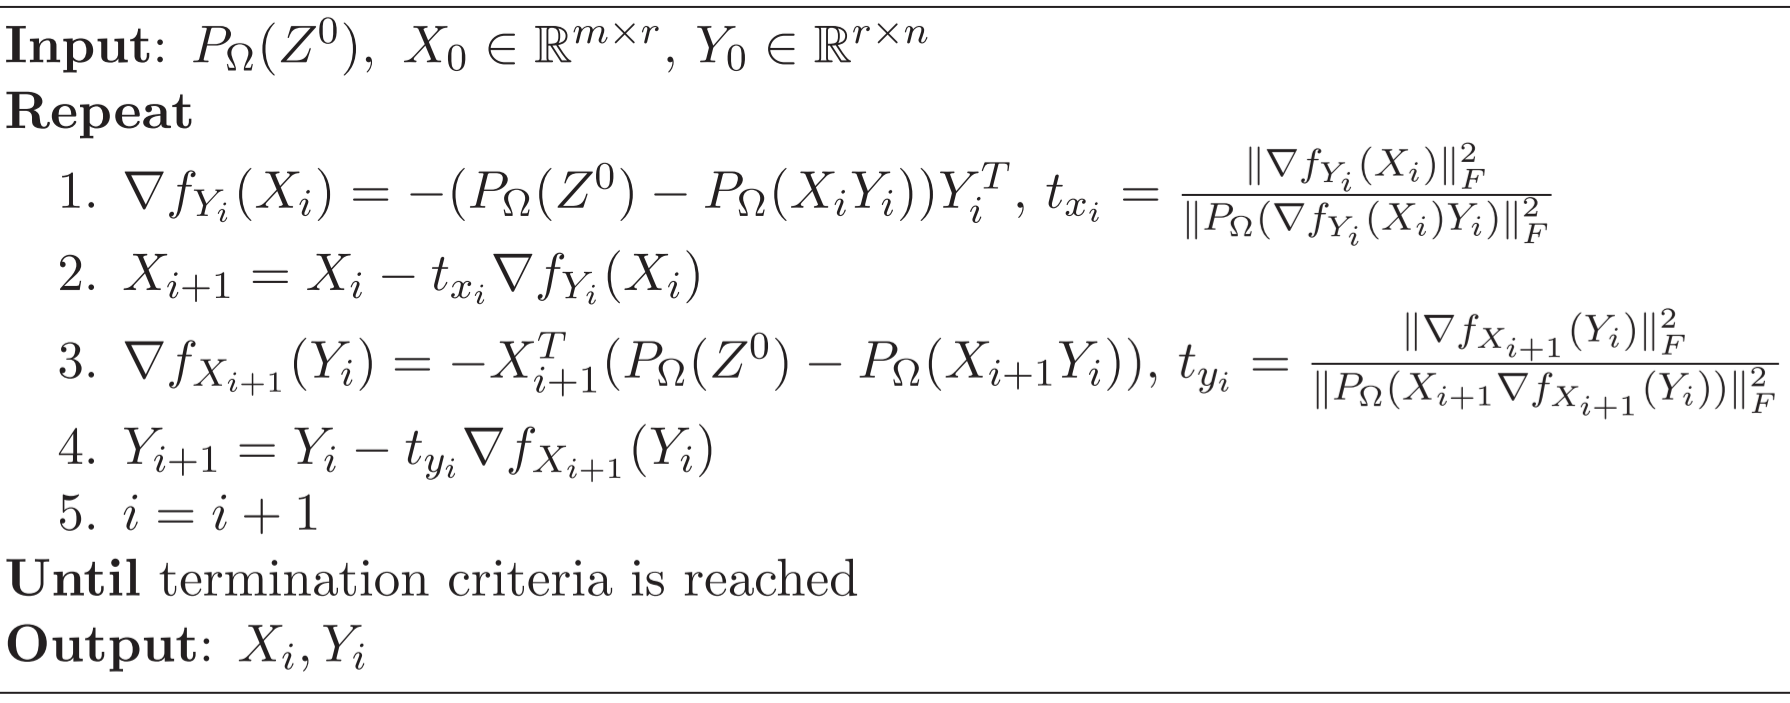
\includegraphics[width=0.95\linewidth]{../Results/ASD_Images/ASD.PNG}
    \caption{Alternating Steepest Descent}\label{fig:ASD}
\end{figure}

\subsection{Actualización eficiente de residuos}
Cuando se actualiza $X_i$ a $X_{i+1}$ hay que recalcular el residuo $P_{\Omega}(Z_0) - P_{\Omega}(X_{i+1}Y)$ y respectivamente lo mismo cuando se actualiza a $Y_{i+1}$. Se puede evitar el costo del producto de matrices con las siguientes propiedades:

\begin{align*}
    P_{\Omega}(X_{i+1}Y_i) &= P_{\Omega}\left( \left( X_i - t_{x_i} \nabla f_{Y_i}(X_i) \right) Y_i \right) \\
                                           &       = P_{\Omega}(X_i Y_i) + t_{x_i} P_{\Omega}\left( \nabla f_{Y_i} (X_i) Y_i \right) \\
    P_{\Omega}(X_{i+1}Y_{i+1}) &= P_{\Omega}\left( X_{i+1} (Y_i - t_{y_i} \nabla f_{X_{i+1}} (Y_i)) \right) \\
                                                 & = P_{\Omega}(X_{i+1}Y_i) + t_{y_i} P_{\Omega}\left( X_{i+1} \nabla f_{X_{i+1}} (Y_i) \right)
\end{align*}

Notemos que las cantidades $P_{\Omega}\left( \nabla f_{Y_i} (X_i) Y_i\right)$ y $P_{\Omega}\left( X_{i+1} \nabla f_{X_{i+1}} (Y_i)\right)$ ya se calcularon antes en los denominadores de $t_{x_i}$ y $t_{y_i}$, por lo que ya no hay que hacer ningún producto matricial.

\subsubsection{Descenso de gradiente alternado escalado}
\label{ssub:escalado}
Presentaremos una versión acelerada del algoritmo de descenso de gradiente alternado. Consideremos el caso en el que todos los valores de la matriz $Z_0$ son conocidas. Bajo esta suposición, podemos simplificar el problema a
\begin{equation*}
    \min_{X, Y} \frac{1}{2} \norm{Z_0 - XY}_F^2
\end{equation*}

Las direcciones del método de optimización de Newton para el problema anterior con respecto a $X$ y $Y$ son
\begin{align*}
    (Z_0 - XY) Y^T (Y Y^T)^{-1} \\
    (X^T X)^{-1} X^T (Z_0 - XY),
\end{align*}
que son las direcciones de máximo descenso escaladas por $(Y Y^T)^{-1}$ y $(X^T X)^{-1}$, respectivamente. Sin embaro, cuando solo una parte de $Z_0$ es conocida, las direcciones de Newton no tienen fórmula explícita como en el caso anterior. Aún así, es posible escalar el descenso de gradiente alternado con $(Y Y^T)^{-1}$ y $(X^T X)^{-1}$. El algoritmo queda como en la figura~\ref{fig:sASD}.

\begin{figure}[htbp]
    \centering
    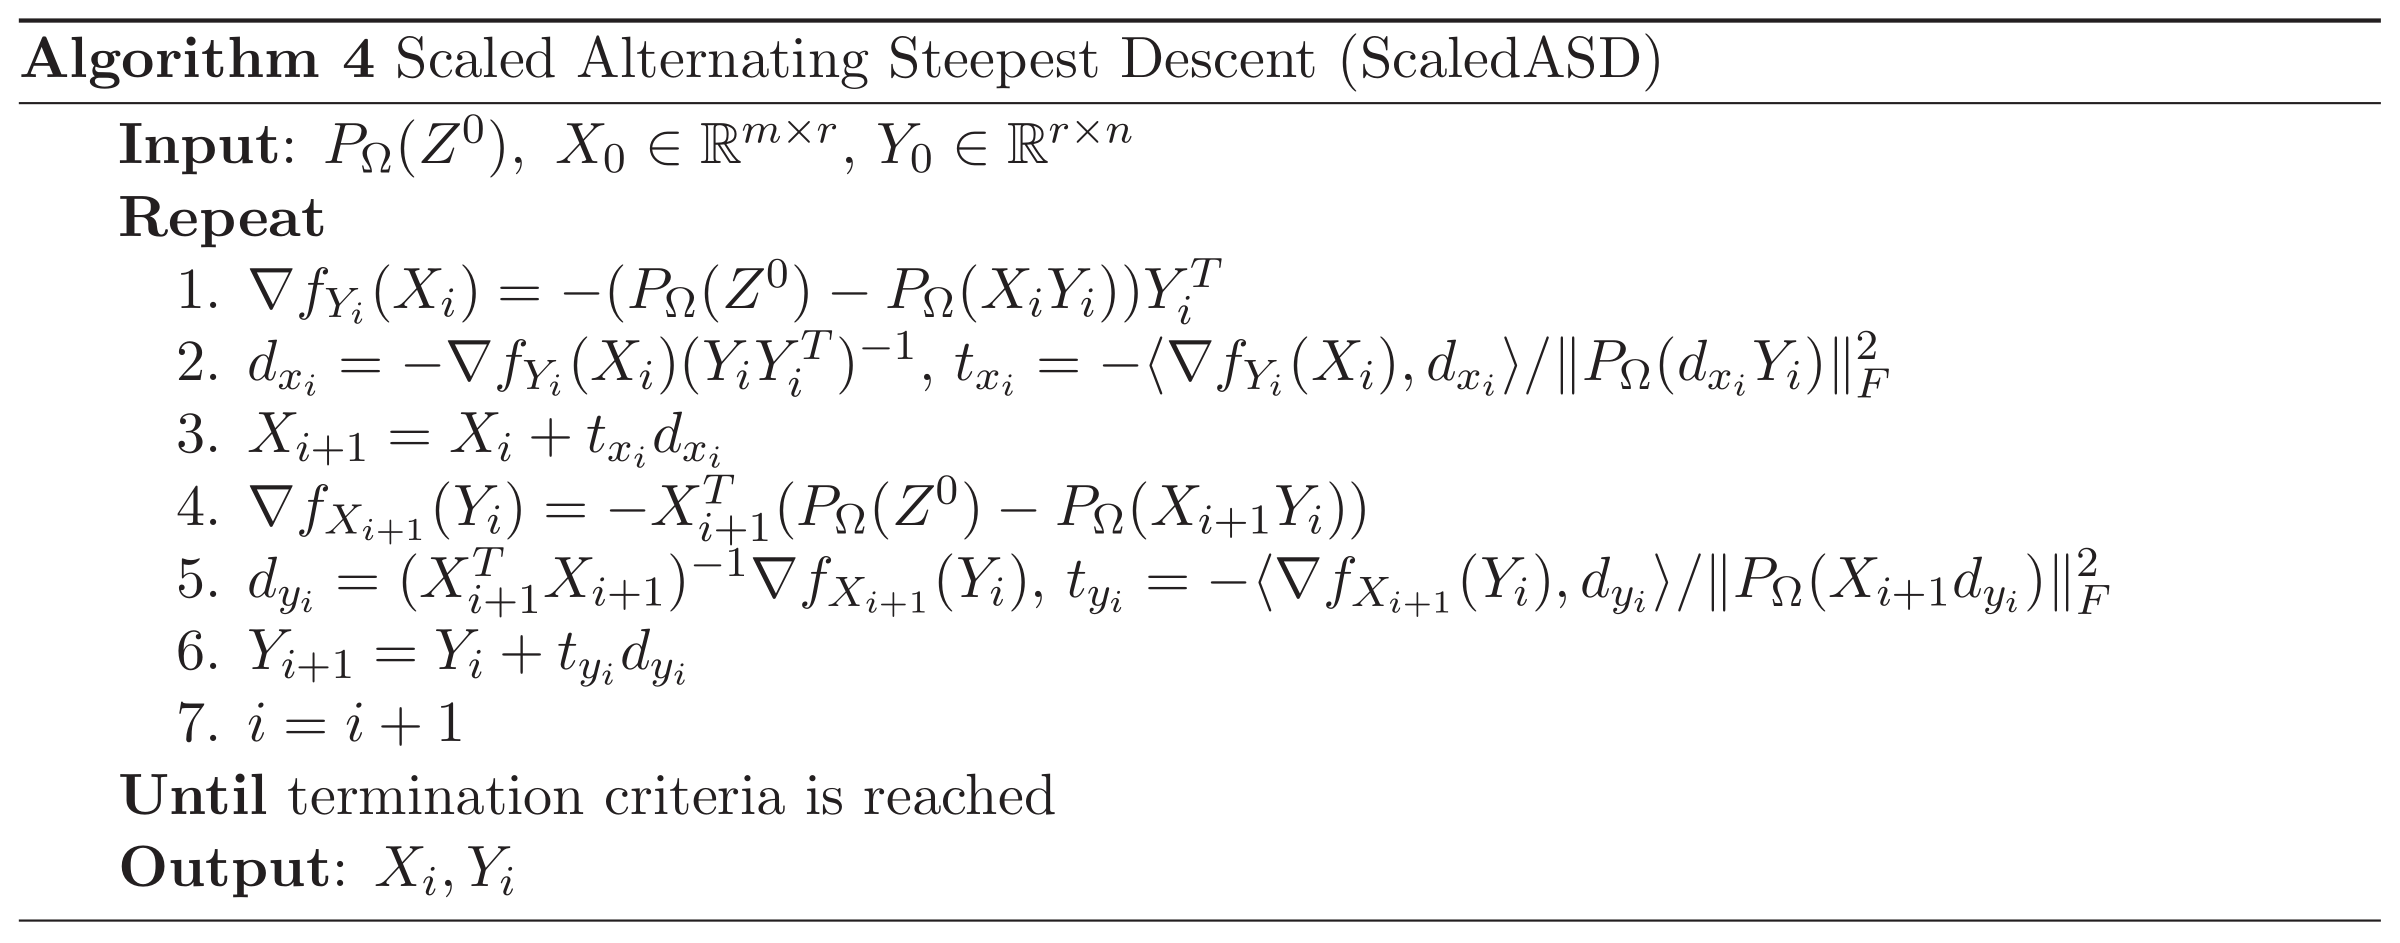
\includegraphics[width=1.0\linewidth]{./Images/sASD_algorithm.PNG}
    \caption{Scaled ASD}\label{fig:sASD}
\end{figure}

\subsection{Experimentos}
Para probar el algoritmo vamos a usar la aproximación de una imagen en blanco y negro con otra imagen, que vista como matriz tenga un rango más bajo. Para esto usamos el siguiente teorema.

\begin{teorema}[Eckart-Young-Mirsky]
    Sea $A \in R^{m \times n}$ con $m\geq~n$ de rango $r$ y sea $A = U \Sigma V^T$ la descomposición en valores singulares de $A$. La matriz de rango $k$ que mejor aproxima a $A$ en la norma de Frobenius está dada por
    \begin{equation*}
        A_k = \sum_{i=1}^{k} \sigma_i u_i v_i^T,
    \end{equation*}
    donde $u_i$ y $v_i$ denotan la $i-$ésima columna de $U$ y $V$, respectivamente.
\end{teorema}

\begin{proof}
    Sea $B \in \mathbb{R}^{m \times n}$ una matriz de rango $k$. Observemos que como $U$ y $V$ son matrices ortogonales
    \begin{align*}
        \norm{A - B}_F^2 &= \norm{U \Sigma V^T - B}_F^2 \\
                         &=\norm{\Sigma - U^T B V}_F^2 \\
                         &=\norm{\Sigma - N}_F^2
    \end{align*}
    donde $N = U^T B V$ es de rango $k$. Expandiendo lo anterior tenemos
    \begin{align*}
        \norm{\Sigma - N}_F^2 &= \sum_{ij}^{} \left( \Sigma_{ij} - N_{ij} \right)^2 \\
                              &= \sum_{i \leq r}^{} \left( \sigma_i - N_{ii} \right)^2 + \sum_{i > r}^{} N_{ii}^2 + \sum_{i \neq j}^{} N_{ij}^2
    \end{align*}
    La expresión anterior se minimiza cuando las entradas de $N$ fuera de la diagonal son cero y $N_{ii}$ son cero para $i > r$. Por último, queda minimizar la primera suma sujeto a que exactamente $k$ de los $N_{ii}$ sean distintos de cero. Esto ocurre cuando $N_{ii} = \sigma_i$ para $i \leq k$ y los demás son cero. Finalmente, de la relación $B = UNV^T$ se obtiene el resultado.
\end{proof}

Utilizamos este algoritmo con 2 imágenes de dimensiones $512 \times 512$, que aproximamos por otras de rango 50. Las imágenes de rango 50 son muestreadas, tomando un $35\%$ de sus entradas de manera uniforme. El resultado de este muestreo es el input del algoritmo, para inicializar las matrices $X$ y $Y$ se utilizan matrices con valores aleatorios enteros entre 0 y 255.

\begin{figure}[htpb]
    \centering
    \subfigure[Rango 507]{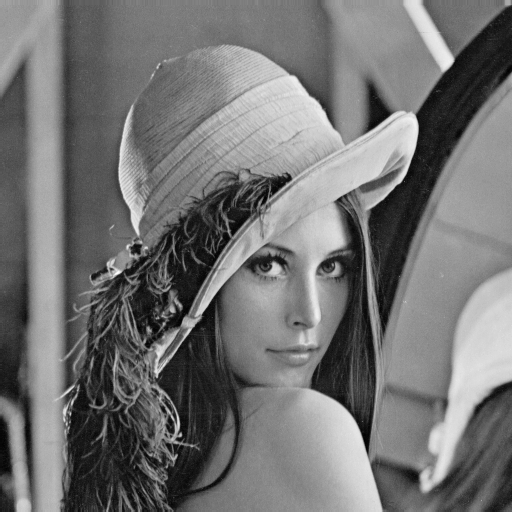
\includegraphics[width=0.3\linewidth]{../Results/ASD_Images/Lena.png}}
    \subfigure[Rango 50]{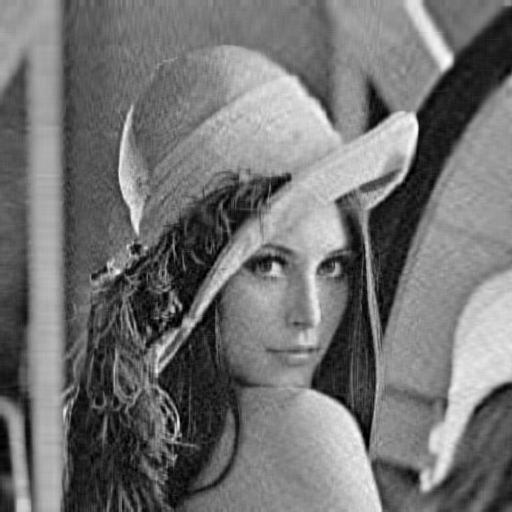
\includegraphics[width=0.3\linewidth]{../Results/ASD_Images/LenaLowRank.png}}
    \subfigure[Muestreo]{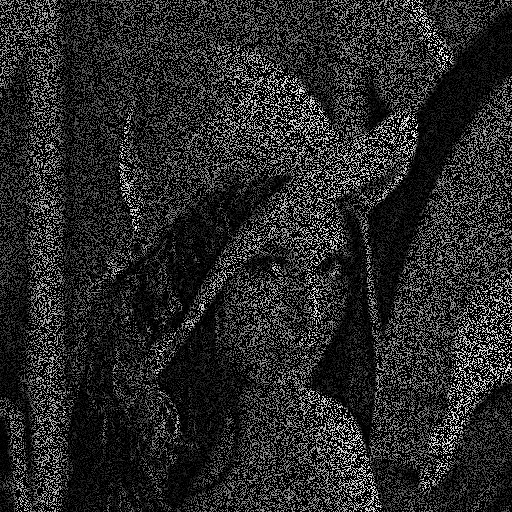
\includegraphics[width=0.3\linewidth]{../Results/ASD_Images/LenaMasked.png}}
    \subfigure[Iteración $10^5$]{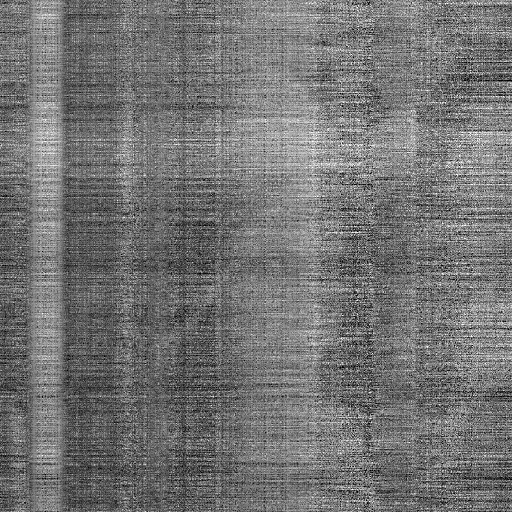
\includegraphics[width=0.3\linewidth]{../Results/ASD_Images/Lena1.png}}
    \subfigure[Iteración $10^6$]{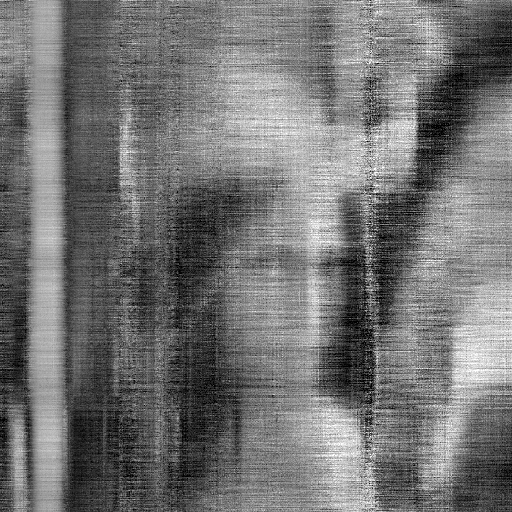
\includegraphics[width=0.3\linewidth]{../Results/ASD_Images/Lena2.png}}
    \subfigure[Iteración $10^7$]{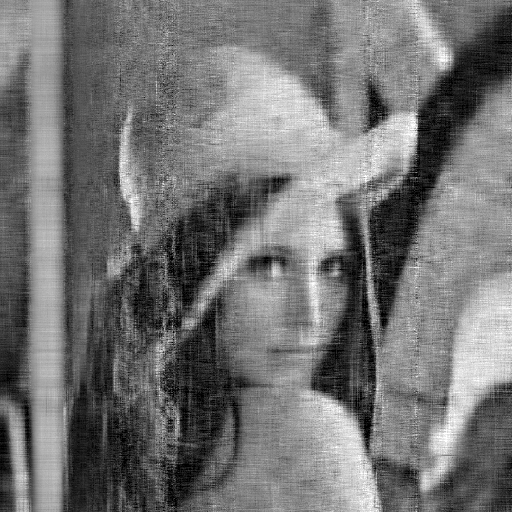
\includegraphics[width=0.3\linewidth]{../Results/ASD_Images/Lena3.png}}
    \caption{Lena}\label{fig:Lena}
\end{figure}

\begin{figure}[htpb]
    \centering
    \subfigure[Rango 512]{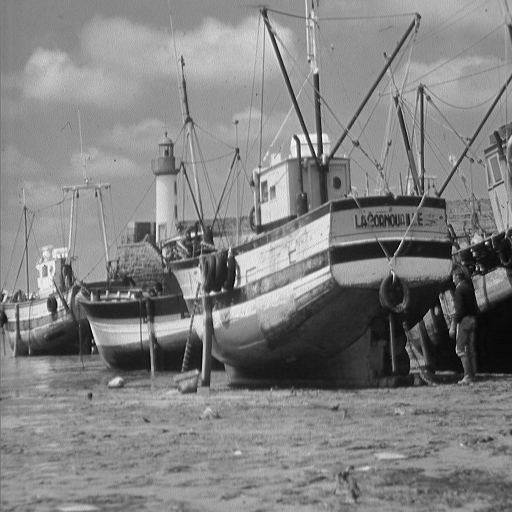
\includegraphics[width=0.3\linewidth]{../Results/ASD_Images/Boat.png}}
    \subfigure[Rango 50]{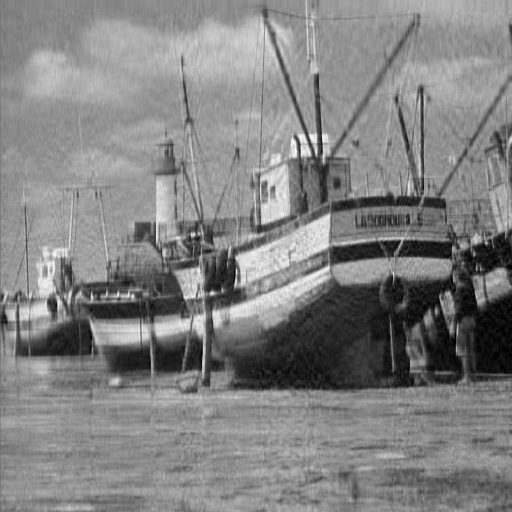
\includegraphics[width=0.3\linewidth]{../Results/ASD_Images/BoatLowRank.png}}
    \subfigure[Muestreo]{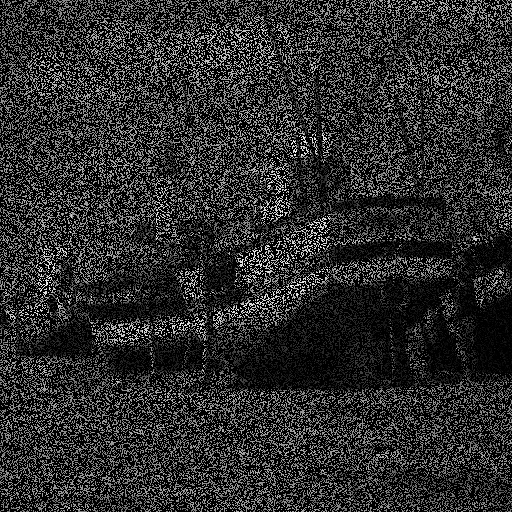
\includegraphics[width=0.3\linewidth]{../Results/ASD_Images/BoatMasked.png}}
    \subfigure[Iteración $10^5$]{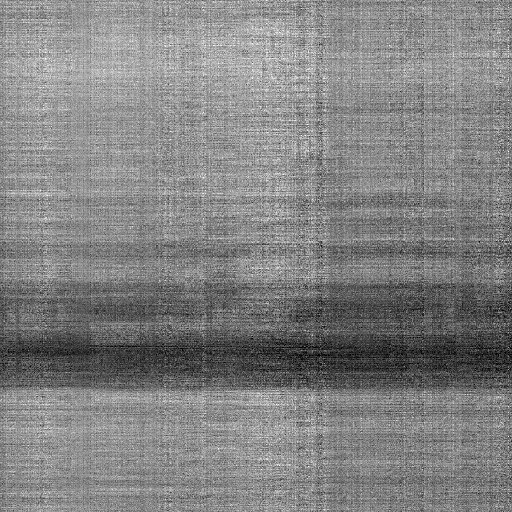
\includegraphics[width=0.3\linewidth]{../Results/ASD_Images/Boat1.png}}
    \subfigure[Iteración $10^6$]{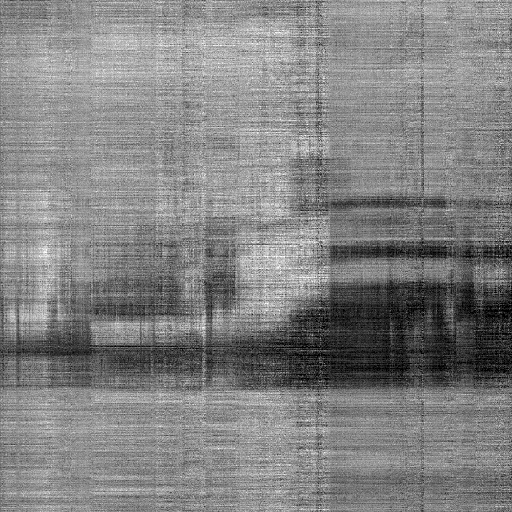
\includegraphics[width=0.3\linewidth]{../Results/ASD_Images/Boat2.png}}
    \subfigure[Iteración $10^7$]{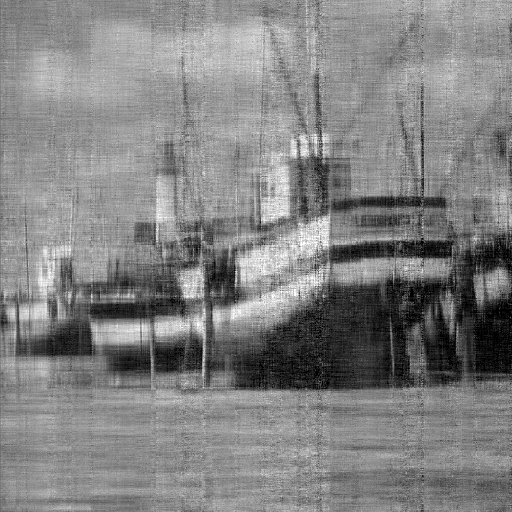
\includegraphics[width=0.3\linewidth]{../Results/ASD_Images/Boat3.png}}
    \caption{Boat}\label{fig:Boat}
\end{figure}

\begin{figure}[htpb]
    \centering
    \subfigure[Original con rango 50]{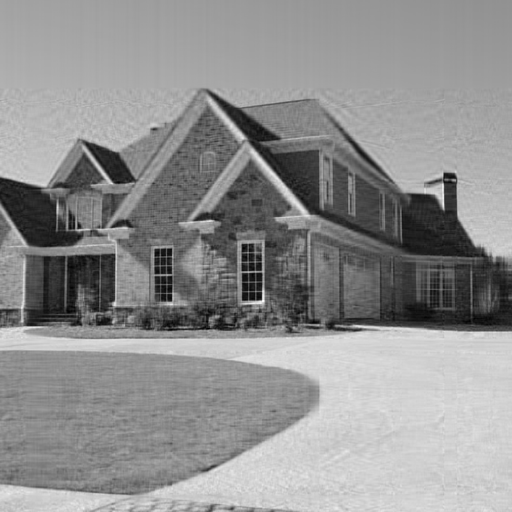
\includegraphics[width=0.3\linewidth]{./Images/House40/low_rank.png}}
    \subfigure[Muestreo del 40\%]{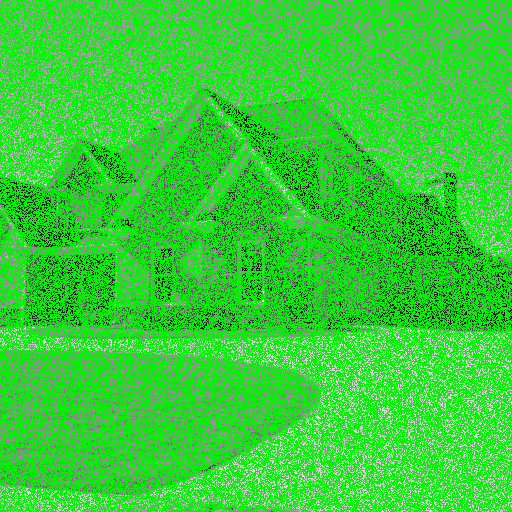
\includegraphics[width=0.3\linewidth]{./Images/House40/masked.png}}
    \subfigure[Aprox. de rango 10]{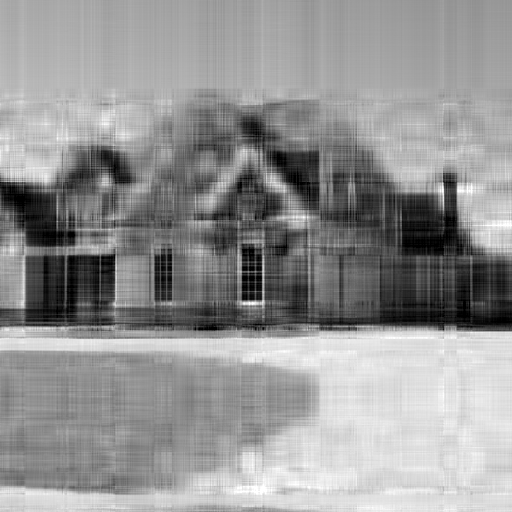
\includegraphics[width=0.3\linewidth]{./Images/House40/pexels-photo-462358__50_10_40_approx.png}}
    \subfigure[Aprox. de rango 20]{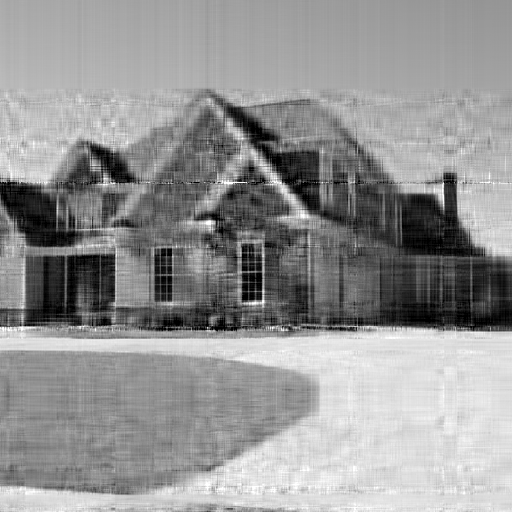
\includegraphics[width=0.3\linewidth]{./Images/House40/pexels-photo-462358__50_20_40_approx.png}}
    \subfigure[Aprox. de rango 30]{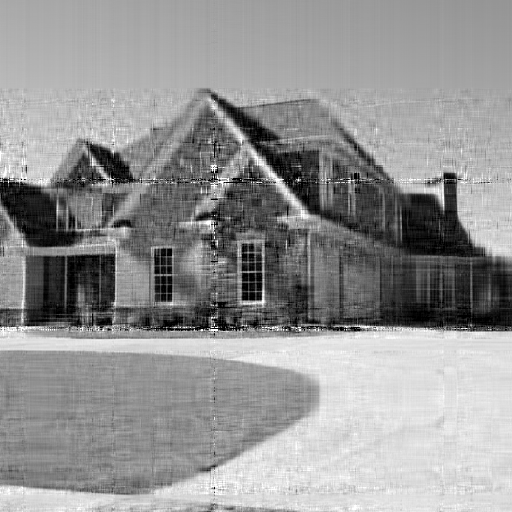
\includegraphics[width=0.3\linewidth]{./Images/House40/pexels-photo-462358__50_30_40_approx.png}}
    \subfigure[Aprox. de rango 40]{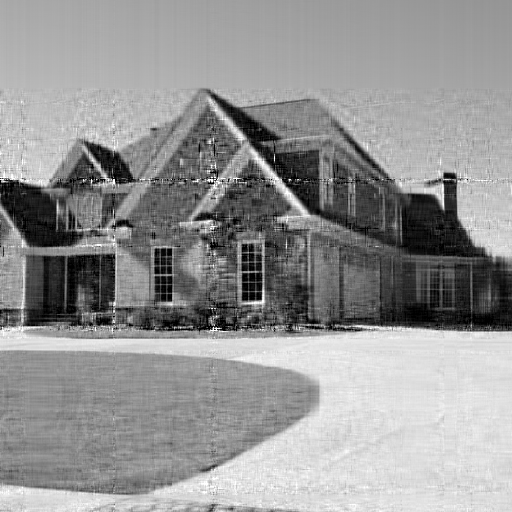
\includegraphics[width=0.3\linewidth]{./Images/House40/pexels-photo-462358__50_40_40_approx.png}}
    \subfigure[Aprox. de rango 50]{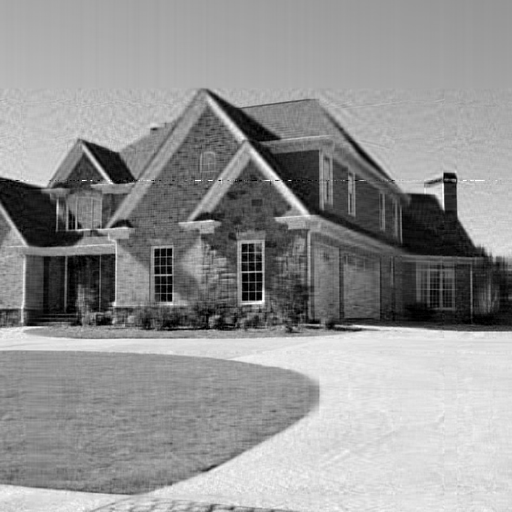
\includegraphics[width=0.3\linewidth]{./Images/House40/pexels-photo-462358__50_50_40_approx.png}}
    \subfigure[Aprox. de rango 60]{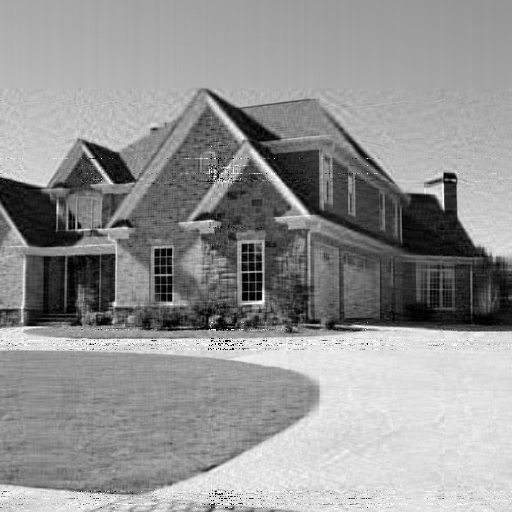
\includegraphics[width=0.3\linewidth]{./Images/House40/pexels-photo-462358__50_60_40_approx.png}}
    \subfigure[Aprox. de rango 70]{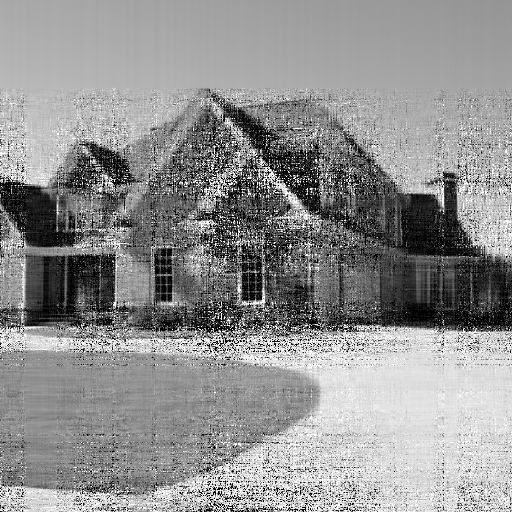
\includegraphics[width=0.3\linewidth]{./Images/House40/pexels-photo-462358__50_70_40_approx.png}}
    \subfigure[Aprox. de rango 80]{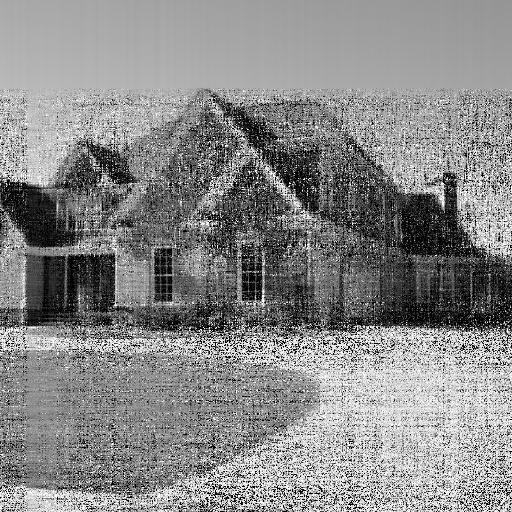
\includegraphics[width=0.3\linewidth]{./Images/House40/pexels-photo-462358__50_80_40_approx.png}}
    \subfigure[Aprox. de rango 90]{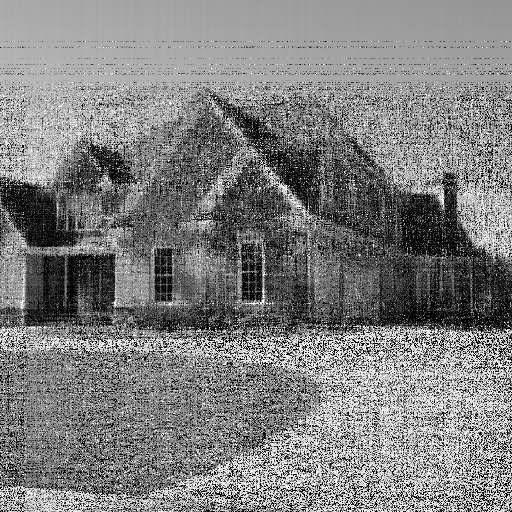
\includegraphics[width=0.3\linewidth]{./Images/House40/pexels-photo-462358__50_90_40_approx.png}}
    \subfigure[Aprox. de rango 100]{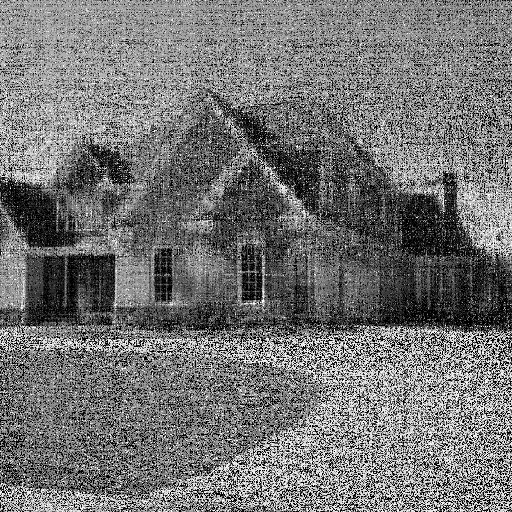
\includegraphics[width=0.3\linewidth]{./Images/House40/pexels-photo-462358__50_100_40_approx.png}}
    \caption{House}\label{fig:House}
\end{figure}

Para las ejecuciones que dieron como resultado las imágenes de las figuras~\ref{fig:Lena}~y~\ref{fig:Boat} el rango real de la imagen fue dado como input al algoritmo, sin embargo el rango real en la mayoría de los casos no es conocido. Dado lo anterior, se hizo otro experimento en el que primero se reduce el rango de una imagen a 50 y después se hace un muestreo del 40\% de los pixeles. Una vez que tenemos el muestreo se ejecuta el algoritmo con distintas propuestas de rango. Como resultado obtenemos las imágenes que se muestran en la figura~\ref{fig:House}. En estas imágenes nos podemos dar cuenta de ciertos patrones:
\begin{itemize}
    \item La mejor aproximación se obtiene cuando el rango propuesto es el mismo que el rango original.
    \item Conforme el rango propuesto se aleja del real, la imagen va teniendo más ruido.
\end{itemize}

Dado lo anterior, una propuesta es hacer búsqueda binaria sobre el rango para obtener la mejor solución sin necesidad de proponer un rango explícitamente.
